\documentclass{exam}

\usepackage{units} 
\usepackage{xfrac} 
\usepackage[fleqn]{amsmath}
\usepackage{cancel}
\usepackage{float}
\usepackage{mdwlist}
\usepackage{booktabs}
\usepackage{cancel}
\usepackage{polynom}
\usepackage{caption}
\usepackage{fullpage}
\usepackage{comment}
\usepackage{enumerate}
\usepackage{graphicx}

\newcommand{\degree}{\ensuremath{^\circ}} 
\everymath{\displaystyle}

% \begin{figure}[H]
%   \centering
%   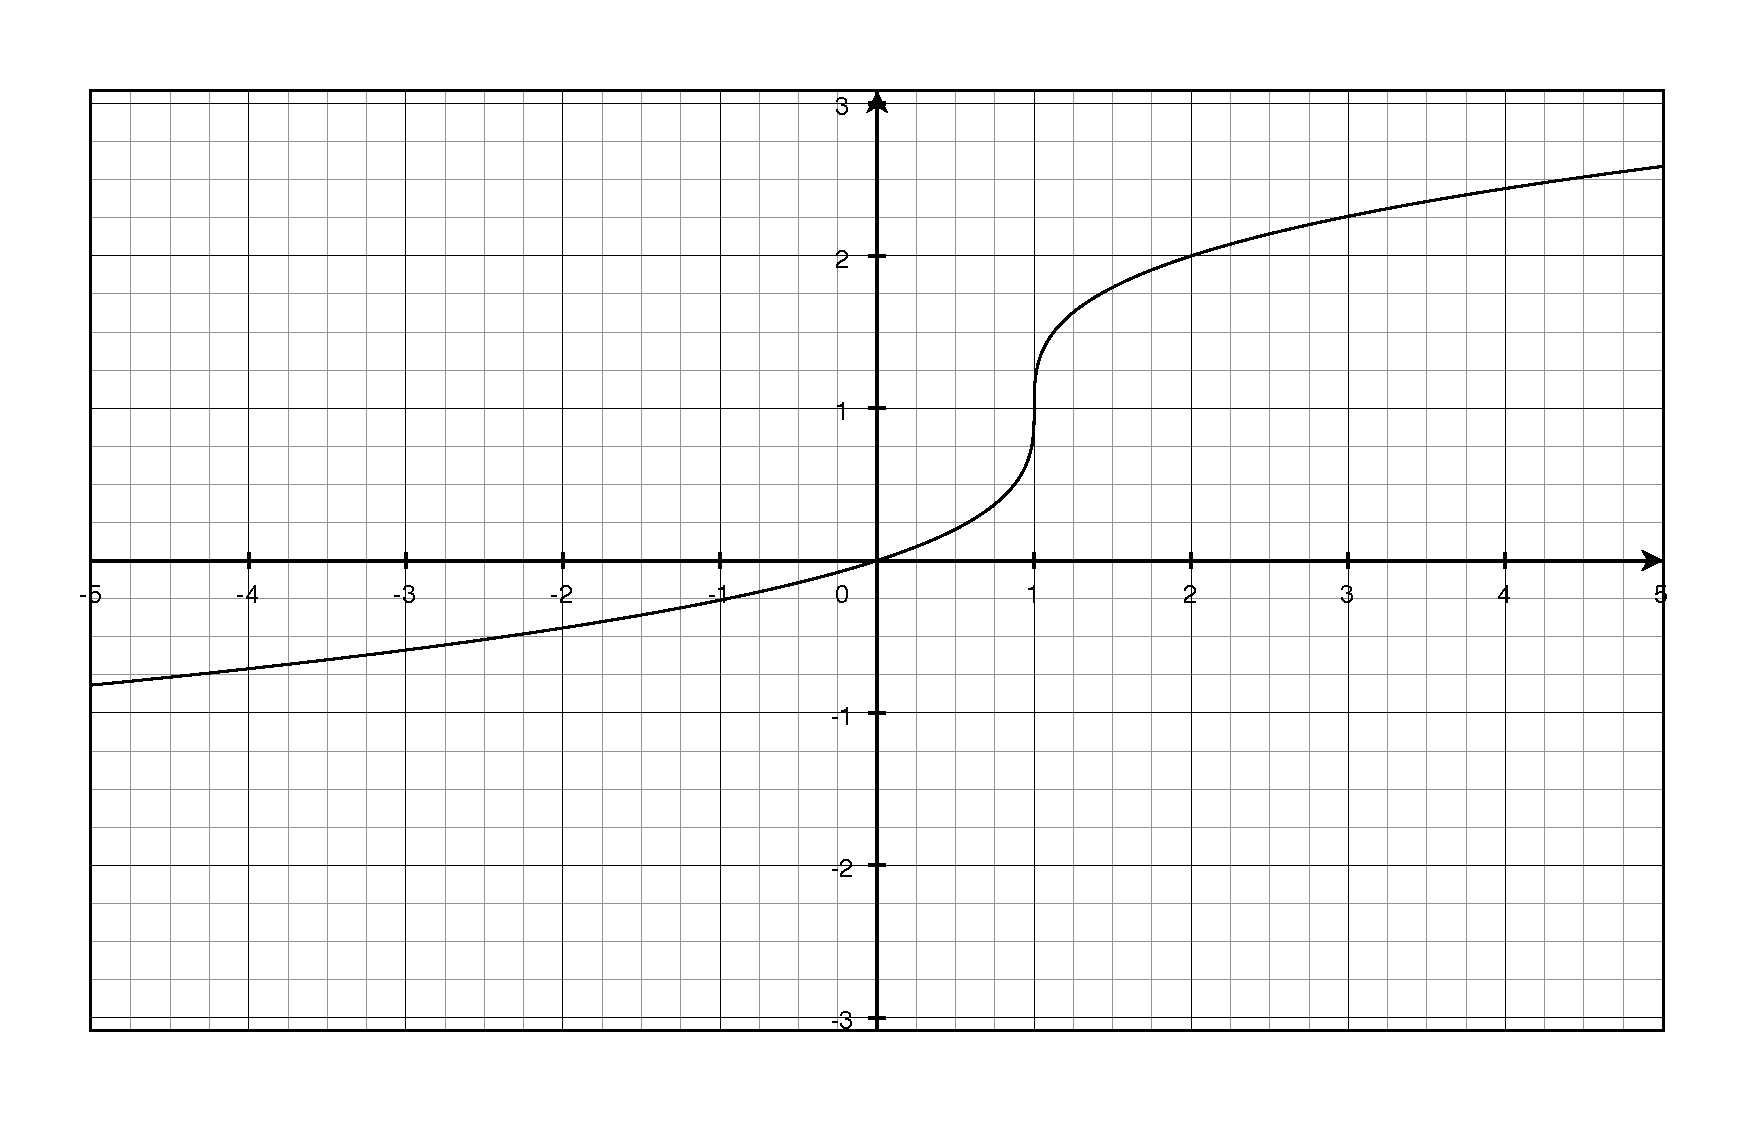
\includegraphics[scale=.3]{question7.eps}
%   \caption*{question 7}
% \end{figure}

\printanswers
\excludecomment{comment}

\ifprintanswers 
  \usepackage{2in1, lscape} 
\fi

\author{}
\date{September 4, 2013}
\title{Math 142 \\ Homework Two}

\begin{document}

  \maketitle

  \section{Homework}
  \begin{itemize*}
    \item read Chapter 1 
    \item do ``Check Your Skills''
    \item hand in exercises: 
  \end{itemize*}

  \section{Extra Credit}

  \ifprintanswers
    \section{Chapter 1}
    \begin{description}

      \item[23]
        \begin{parts}
          \part categorical
          \part categorical
          \part quantitative
          \part categorical
          \part quantitative
        \end{parts}

      \item[24]
        \begin{parts}
          \part David Ortiz, Laynce Nix, Antonio Perez, Mike Piazza, and Scott Rolen
          \part team, position, age, height, weight, salary
          \part years, feet and inches, pounds, dollars
        \end{parts}

      \item[26]
        \begin{figure}[H]
          \centering
          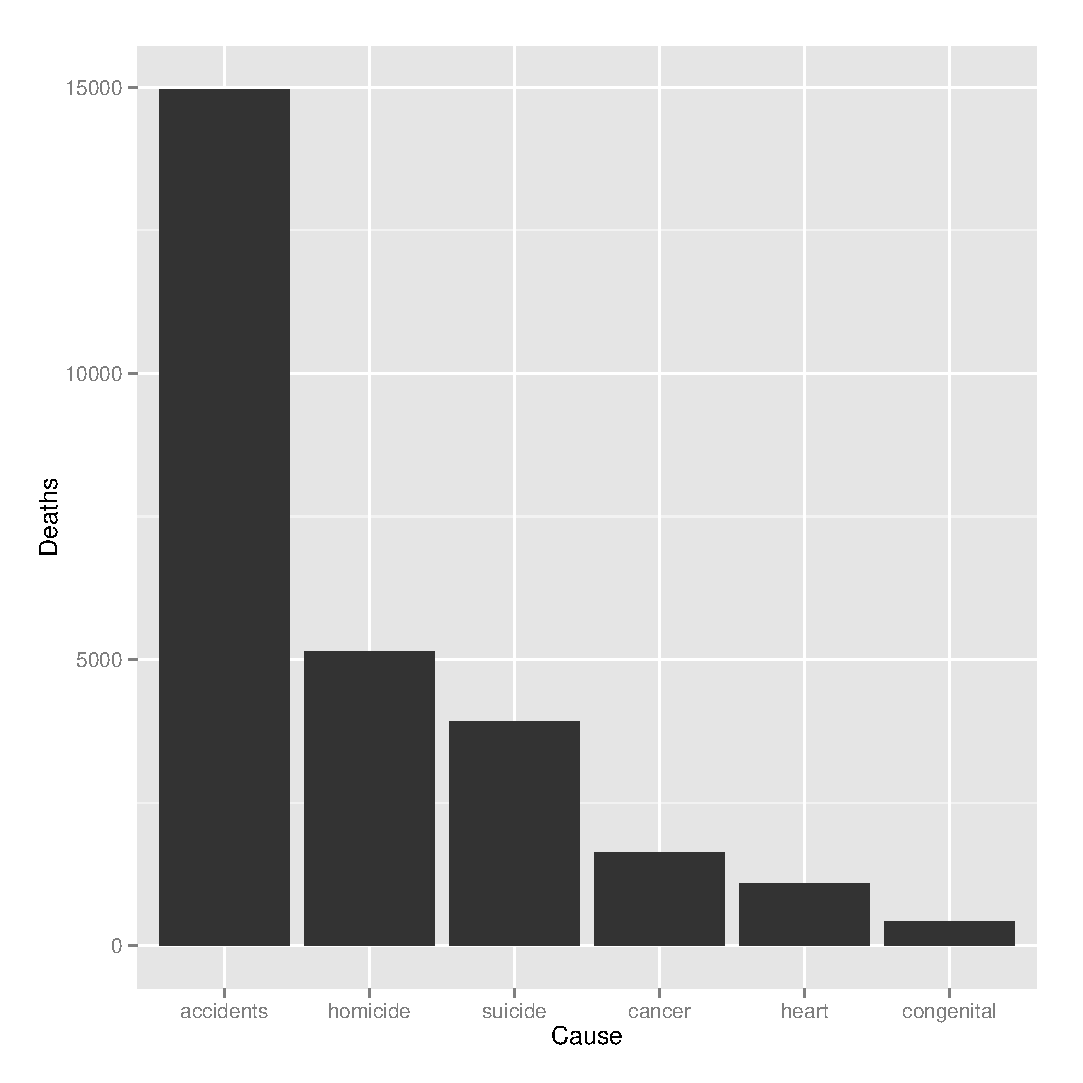
\includegraphics[scale = 0.5]{ex26.eps}
          \caption{Exercise 26}
        \end{figure}
    \end{description}

  \else
    \vspace{9 cm}
    \begin{quote}
      \begin{em}
      \end{em}
    \end{quote}
    \hspace{1 cm} --TO DO
  \fi

\end{document}

